\section{schmierzettel:}

Aufgabenstellungen zu der DSL:



\section{DSL}

% Programmierer entwickeln Software überwiegend in universell einsetzbaren
% Programmiersprachen (engl.
% general purpose language, GPL), wie z.B. Java, C\#.
% Diese Sprachen sind, für nahezu jeden Anwendungszweck einsetzbar.
% Dadurch werden diese Sprachen komplex und deren Benutzung ist nur durch gut
% ausgebildete Programmierer möglich.
% Programmierer bilden Sachverhalte, Objekte und Prozesse aus der realen Welt
% mit Hilfe einer Kombination der universell einsetzbaren Konstrukte
% aus der Programmiersprache ab.
% Zur Erstellung benötigen die Entwickler Spezifikationen, die die zu erstellende
% Software genau beschreiben. Diese werden widerrum von Experten erstellt, deren
% Job es ist mit den Auftraggebern bzw. den Domänenexperten zu kommunizieren, um
% daraus eine Spezifikation abzuleiten. Diese Spezifikation ist der sogenannte
% Problemraum. Die Erstellte Software ist der Lösungsraum. 
% Um die Spezifikation wäerend oder nach der Entwicklungsphase zu verifizieren
% sind Tests notwendig.



%TODO start copy--
% Diese Art der Softwareentwicklung führt in der Praxis zu verschiedenen Proble-
% men. Es entstehen hohe Aufwände für Spezifikation und Test. Trotzdem ist die
% entwickelte Software häufig fehleranfällig und entspricht oft nicht genau den
% Spezifikationen. Nachbesserungen sind nötig, die Geld und Zeit kosten.
%  
% Domänenspezifische Sprachen können in bestimmten Situationen helfen, um diesen
% Problemen zu begegnen. Die grundsätzli- che Idee ist, ausgewählte Softwareteile
% nicht mehr mit universell einsetzbaren Programmiersprachen zu entwickeln, son-
% dern stattdessen Sprachen zu benutzen, die auf die konkrete Anwendungsdomäne
% spezialisiert sind. Der Quelltext, der mit einer solchen Sprache entwickelt
% wird, kann später vollautomatisch in den Quell- code einer universellen
% Programmierspra- che übersetzt werden. Der Vorteil ist, dass der Sprachumfang
% der DSL aufgrund der Spezialisierung auf eine Domäne im Vergleich mit einer
% universellen Sprache viel kleiner ist. Um domänenspezifische Sachverhalte als
% Quellcode auszudrücken ist deutlich weniger Zeit und Quellcode nötig, zur
% Programmierung reicht oft das  Domänenwissen des Anwendungsexperten aus. Im
% Extremfall könnte statt dem Programmierer der Anwendungsexperte das benötigte
% Programm schreiben. Die Erstellung des DSS-Quellcodes erfolgt mittels eines
% speziellen Editors, der die Sprachelemente als Textbefehle oder durch grafische
% Elemente bereitstellt.
% Ein solcher Editor kann so definiert werden, dass er, entsprechend den Vorgaben
% der Anwendungsdomäne, nur vorher festge- legte Kombinationen von Sprachelemen-
% ten zulässt und damit der Sicherstellung fachlicher Rahmenbedingungen besonders
% Rechnung trägt.
% 
% 
% Eine DSL ist in der Regel nicht dazu geeignet, komplette Anwendungen zu gene-
% rieren. Vielmehr sollte ein DSL zur Entwicklung kleinerer Anwendungsteile, die
% bestimmte Eigenschaften erfüllen, benutzt werden. Besonders sinnvoll ist der
% Einsatz einer DSL für Softwareteile, die häufig änderungen unterliegen. Dies
% ist zum Beispiel bei Produktdefinitionen, Verarbei- tungsregeln, Tarifrechnern
% und ähnlichem oft der Fall. Weiterhin sollte eine DSL nicht für Software
% verwendet werden, an die sehr hohe Performanceanforderungen gestellt werden.
% \cite{uniLeipzigTechRadar}
% % TODOD end copy ---


\section{groovy metaprogramming}


%TODO sind lisp macros auch metaprogrammierung?

% Metaprogrammierung ist eine Programmiertechnik, die Codegenerierung einsetzt, um
% bessere Abstraktion zu ermöglichen.
% Ein Evaluierer bestimmt den Wert eines formalen Ausdrucks. Z.B. ist der Wert des
% formalen Ausdrucks “5 + 3” “8”. Für Metaprogrammierung ist es oft nötig
% formale Ausdrücke zur Lauf- zeit auswerten zu können. Programmiersprachen wie
% Ruby oder Lisp stellen hierfür einen Eva- luierer über eine eval-Funktion
% bereit.
% Linguistische Abstraktion bezeichnet Abstraktion auf linguistischem
% Sprachniveau. Dabei be- zeichnet hier der Begriff “Sprache” primär formale
% Sprachen.
% Metalinguistische Abstraktion ist Abstraktion auf (linguistischem) Sprachniveau,
% die den Evalu- ierer umschreibt oder einen eigenen Evaluierer verwendet. Ein
% Beispiel ist ein lazy eval für eine strikt ausgewertete Sprache wie etwa Java.
% Der Begriff der Metalinguistischen Abstraktion ist nicht klar definiert und eine
% harte Abgrenzung zu anderen Konzepten (etwa Frameworks) vorzu- nehmen ist kaum
% möglich.
% Metaprogrammierung kann man als Werkzeug verstehen, das linguistische
% Abstraktion erzeugt.(vgl. \cite{biekermetaprogrammierung})
% 
% Metaprogrammierung bezeichnet eine Programmier-Technik um Code automatisch zu
% generie- ren. Es geht also um Code der Code schreibt.
% Der Ursprung der Metaprogrammierung geht auf das 1958 am MIT entwickelte Lisp
% bzw. Sche- me zurück. In Lisp gibt es (defmacro ..) und in Scheme (define-syntax
% ..) Makros. Ein Lisp-Makro ist einer Funktion ähnlich. Eine Funktion erhält
% Parameter und liefert einen oder mehere Werte zurück. Ein Lisp-Makro erhält
% Parameter und liefert einen oder mehere Code- Ausdrücke zurück, die wieder
% evaluiert werden.
% Vor der Entwicklung der Lisp-Makros gab es bereits selbstmodifizierenden
% Assembler-Code. Das Problem hiermit ist das zu niedrige Abstaktionsniveau, da
% man sich auf Opcode-Ebene mit der Manipulation des Codes beschäftigen muss.
% In Ruby gibt es die Methoden define method und define class, mit der man
% Methoden bzw. Klassen definieren kann. Um Metaprogrammierung betreiben zu
% können, ist es essentiel, dass man solche Funktionen hat, damit man dynamisch
% Methoden und Klassen erzeugen kann. Des Weiteren stellt Ruby eval Funktionen zur
% Verfügung, mit denen Code in unterschiedlichen Kon- texten ausgeführt werden
% kann.
% InRubywirdkomplexereMetaprogrammierungüberInterpreter-Hooksrealisert,etwamethodmissing.
% method missing wird augerufen, wenn man eine nicht vorhandene Methode auf einem
% Objekt
% aufruft.DieDefault-ImplemtierungwirfteineNoMethodErrorException.Durchüberschreiben
% dieser Method kann man z.B. ein Dateisystem Objekt erzeugen, dass als
% Methodenaufrufe sei- ne Unterordner kennt. Dies ermöglicht es z.B. ein
% Verhalten, analog zu dem Shell-Befehl cd dirname, über fsobj dirname zu
% realisieren.
% Ein anderer Interpreter-Hook ist Class.inherited, der immer ausgeführt wird,
% wenn man von einer Klasse erbt. Möchte man verhindern, dass von einer Klasse
% geerbt wird, kann man in Class.inherited eine Exception werfen.
% 
% Oft wird Metaprogrammierung als eine Form der Codekomprimierung verstanden. Es
% geht bei Metaprogrammierung nicht um das reine Einsparen von Zeichen bzw. Code-Zeilen, sondern um Abstraktion.
% 
% (vgl. \cite{biekermetaprogrammierung})
% 
% Introspection bezeichnet die Fähigkeit, auf Informationen über die Zustäe
% von Objekte, deren Klassen und Verhalten zur Laufzeit zugreifen zu können.
% Intercession erlaubt Zustände und Verhalten von Objekten, aber auch deren
% Klassen zur Laufzeit zu verändern. Intercession setzt meist Introspection
% voraus.\cite{mpInGroovy}
% 
% \section{probleme und loesungsansaetze} 
% Ich beschreibe nun einige Probleme mit Metaprogrammierung und DSLs. Es geht mir
% hier nicht um Vollständigkeit, sondern darum einige Probleme und potenzielle
% Lösungen auf zu zeigen.
% Eins der wichtigsten Probleme ist die hohe Komplexität. In [Diomidis Spinellis.
% Rational metaprogramming. IEEE Software, 25(1):78–79, January/Fe- bruary 2008.]
% beschreibt der Autor das Pro- blem wie folgt:
% “While I admire the cleverness and skill that hides behind C++ libraries (...),
% the fact remains that writing advanced template code is devilishly hard, (...)”
% Die Komplexität lässt sich durch die Verwendung bekannter Metaprog. Paradigmen
% und Patterns reduzieren. Lisp hat hier etliche zu bieten, etwa defmacro,
% Higher-Order Functions oder Currying.
% Eine DSL bzw. ein Metaprogammierungsframework sollte im mathematischen Sinne
% abgeschlos- sen sein. D.h. man soll den selben Code erzeugen können, den man von
% Hand schreiben kann und umgekehrt.
% Komplexe DSLs erzeugen teilweise schwer debugbaren Code. Nach Wissensstand des
% Autors gibt es zur Zeit kaum Lösungsansätze für dieses Problem.
% Es bleibt nur anzumerken, dass auch komplexe Frameworks teilweise schwer
% debugbaren Code erzeugen.
% Eine häufige Quelle für schwer debugbaren Code ist es, den Code als String
% darzustellen und dannzuevaluieren.Diesf ührt oft zu sinnfreien Fehlermeldungen
% wie “Syntax error in line 1 at char 42’’, wobei der evaluierte Code an anderer
% Stelle steht. Ruby und viele andere Sprachen bieten Konstrukte an, die es nicht
% zulassen, dass man syntaktisch falschen Code er- zeugt. In Ruby kann man hierfür
% Blöcke verwenden.
% Ein anderes Problem ist die Sprachkonsistens. Es ist schwierig gute und
% konsistente Sprachen zu erzeugen. Es ist aufwändig diese Sprachen zu lernen und
% ihr Support ist ressourcen-intensiv. Es macht daher Sinn die neue Sprache
% möglichst gut in die vorhandene Sprachumgebung ein zu gliedern. Eingebettete
% DSLs helfen hierbei.
% (vgl. \cite{biekermetaprogrammierung})
\section{kategorien}


% Mit Kategorien bietet Groovy eine Art dynamische Mix-ins. Es können innerhalb
% von einem Closure, beliebige Methoden zu allen Metaklassen hinzugefügt oder
% überschrieben werden.
% Die Methode use ist eine der Standardmethoden in DefaultGroovyMethods die jeder
% Metaklasse, die von MetaClassImpl erbt, automatisch hinzugefügt wird. Deswegen
% wird häufig von use auch von einem Sprachkonstrukt statt von einer Methode
% gesprochen. Mit use wird die in Klammern angegebene Klasse auf Klas- senmethoden
% untersucht und in org.codehaus.groovy.runtime.GroovyCategory- Support verwaltet.
% Es werden nur Klassenmethoden erlaubt, um Zustände in der Kategoriein- stanz zu
% vermeiden, die nicht threadsicher wären. Der this Parameter wird des- halb bei
% Üerschreiben von Instanzmethoden wie getName explizit als ersten Parameter
% angegeben. Wird nun eine Methode aufgerufen, überprüft MetaClas- sImpl in
% invokeMethod ob es eine Kategorie Methode gibt, die kompatibel ist mit dem
% aktuellen Objekt und den übergebenen Parametern. Gibt es solch eine wird der
% Aufruf delegiert, sonst wird wie in 2.5 beschrieben der normale Aufruf
% fortgesetzt.
% Kategorien sind von Objective-C entlehnt und bieten eine einfache Mög-
% lichkeit, kurzzeitig und ohne Seiteneffekte neue Methoden hinzuzufügen oder
% bestehende zu überschreiben. Sie eignen sich deswegen gut für Aspekt- oder
% Contextorientierte Programmierung. \cite{mpInGroovy}
% \subsection{Expando-MetaClass}


\section{Metaprogrammierung in Groovy}

% 
% 
% Groovy besteht aus einem flexiblen Metaklassenmodell. Im Sinne einer Open
% Implementation hat der Programmierer nahezu alle Möglich- keiten sein Programm
% mittels Reflection zur Laufzeit zu verändern und damit an die individuellen
% Bedürfnisse anzupassen. \cite{mpInGroovy} Da Groovy auf der Java VM ausgeführt
% wird und somit auch den Grundregeln des Javaklassenmodells folgen muss,
% unterliegt es auch dessen Einschränkungen. In Java ist eine Veränderungen der
% Klassen zur Laufzeit nicht vorgesehen. Die Java Runtime Environement stellt mit
% dem java.reflect Package primär eine Mölichkeit zur Introspection bereit.
% [\ldots] 
% Erst Javassist, und Reflex erlauben echtes dynamisches
% Verhalten, in dem auf Byteco- de Ebene die Klasse verändert wird. 
% 
% Dazu muss allerdings die Klasse teilweise umständlich entladen und neugeladen
% werden. 
% Ein Meta Object Protocol auf der Java VM kann
% somit nur mittels einer zusätzlichen Indirektionsschicht realisiert werden.
% Dazu werden bestehende Konzepte von Java benutzt und um ein Metaklassenmodell
% erweitert. Aus dem Java Unterbau ergeben sich folgende Grundsätze:
% Wie in Java ist in Groovy jede Klasse abgeleitet von Object. Groovy ist in
% diesem Hinblick aber wesentlich konsequenter, da auf primitive Datentypen
% bewusst verzichtet wurde, um die Inkonsistenzen bei der Behandlung von pri-
% mitiven Datentypen und Klassen zu vermeiden. Weiterhin ist jede Klasse in Groovy
% eine Instanz von Class, womit Class alsöauch in Groovy die Klasse der Klassen
% bleibt.  \cite{mpInGroovy}
% 
% \paragraph{ getMetaClass setMetaClass} Nicht nur eine Klasse hat eine
% Metaklasse, sondern auch jedes einzelne Groovy Objekt kann eine von der Klasse
% unabhängige Metaklasse haben (siehe 2.4). Diese instanz- spezifische Metaklasse
% ist über die beiden Methoden zugänglich.\\
% 
% \paragraph{ getProperty setProperty} Properties definieren den Zustand eines
% Objektes und werden in Groovy primär auf Instanz und Klassenebene abgebildet. Jede Groovy
% Klasse kann durch Überschreiben dieser zwei Methoden dynamische Properties auf
% Objektebene oder Klassenebene erzeugen. \\
% 
% \paragraph{ invokeMethod } Das Verhalten eines Objektes ist wiederum eine Ebene
% höher angesiedelt, spielt sich alsöauf Klassen- oder Metaklassenebene ab.
% Normalerweise wird dynamisches Verhal- ten damit auf Metaklassenebene
% realisiert, sodass diese Methode der GroovyObjects gar nicht erst aufgerufen
% wird. Nur im Fehlerfall oder mit Hilfe des Tag-Interfaces GroovyInterceptable
% wird invokeMethod aufgerufen (in 2.5 genau beschrieben).
% 
% [\ldots] Während GroovyObject dynamisches Verhalten auf Objekt- und
% Klassenebene erlaubt, ist das zweite elementare Interface MetaClass die Grund-
% lage für das sehr ausgewogene Metaklassenmodell in Groovy.
% 
% \paragraph{ Metaklassen, Klassen und Instanzen} Läuft ein Programm ohne
% Intercession, sögelten für die Metaklassen der Klassen und Instanzen folgen- de
% Grundaussagen: Jede Klasse hat eine Metaklasse, die eine Instanz von Me-
% taClassImpl ist und damit MetaClass implementiert. Diese Instanzen werden
% dynamisch erzeugt und sind bis auf wenige Ausnahmen direkt MetaClassImpl
% Instanzen. Java Klassen erhalten eine Instanz von ExpandoMetaClass als Meta-
% klasse, damit auch diesen Klassen Methoden hinzugefügt werden können. Neue
% Instanzen von Klassen werden über die Metaklasse der Klasse erstellt und haben
% diese Metaklasse als Metaklasse.
% 
% 
% 
% 
%  
% \paragraph{ getProperties getMethods getMetaMethods}
% Die Methoden der Introspection in Groovy. Der Unterschied zwischen getMethods
% und getMetaMethods wird in 2.5 näher erläutert.
% \paragraph{ getClassNode}
% Liefert den AST der Metaklasse sofern verfügbar. Erlaubt auch die Modifikation
% dieses ASTs und ist damit sowohl für Introspection als auch Intercession
% geeignet. Aufgrund der Komplexität des ASTs wird allerdings dynamisches
% Verhalten häufiger über die ExpandoMetaClass realisiert und der AST verwendet,
% um Quelltextfragmente neu zu interpretieren. In den Standardbibliotheken wird so
% zum Beispiel eine Closure auto- matisch in ein SQL Statement umgewandelt, um das
% SELECT Statement performant zu benutzen.
% \paragraph{ invokeMethod}
% Jeder Methodenaufruf wird primär von der Metaklasse behandelt und entweder an
% die invokeMethod Funktion des GroovyObjects oder aber an die entsprechende
% Methode der Klasse delegiert. Das Erzeugen einer eigenen Metaklasse und
% überschreiben dieser Methode ist die Hauptmöglichkeit für dynamisches
% Verhalten in Groovy außer der ExpandoMetaClass.
% \paragraph{ getProperty setProperty}
% Die Methoden zur Property-Unterstützung auf Metaklassenebene werden von der
% Standardimplementierung von den entsprechenden Methoden von GroovyObject auf-
% gerufen. Die Aufrufreihenfolge ist im Vergleich zu invokeMethod alsögenau
% anders- herum. Auch diese Methoden sind für Intercession geeignet.
% \paragraph{ invokeMissingMethod invokeMissingProperty}
% Diese Backupmethoden werden jeweils aufgerufen, wenn die normalen Aufrufmecha-
% nismen fehlgeschlagen sind. Intercession mit diesen Methoden erlaubt zum
% Beispiel die Erweiterung von Klassen und Objekten um zusätzliche Properties zur
% Laufzeit.
%  \cite{mpInGroovy}
% 
% 
% \begin{figure}[h!]
% 	\begin{center}
% 	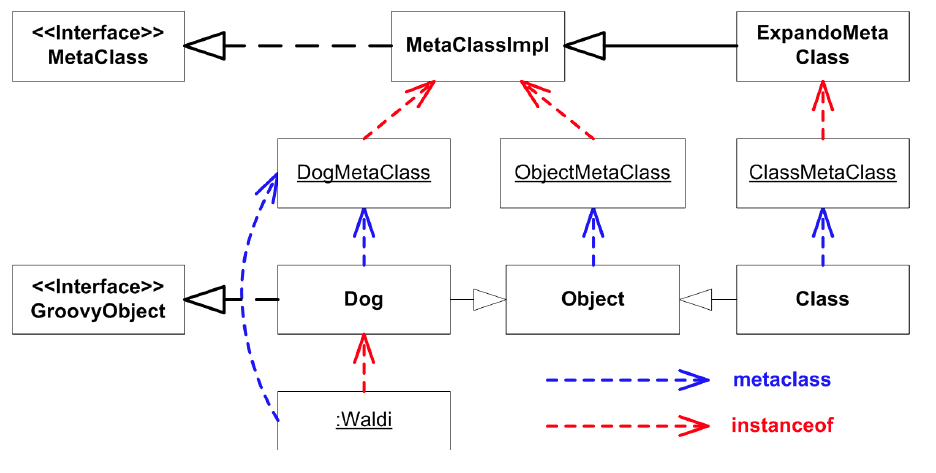
\includegraphics[width=0.8\textwidth]{pics/groovyMetaklassen}
% 	\end{center}
% 	\caption{Beziehung von Metaklassen, Klassen und Instanzen \cite{mpInGroovy})}
% 	\label{groovyMetaclassDiagram}
% \end{figure}

 

 
 

\chapter{Zusammenfassung und Schlussbetrachtung}

 %begin copy -- unterschiede dsm und mda
% Domänenspezifische Modellierung erlaubt schnellere Entwicklung
% basierend auf den Modellen der Problemdomäne und weniger auf
% Modellen von Quellcode. Unser Uhrenbeispiel veranschaulichte dies
% schnell. Industrielle Erfahrungen mit DSM [DSM] zeigen bedeutende
% Verbesserungen der Produktivität, niedrigere Entwicklungskosten
% und bessere Qualität. Das Unternehmen Nokia gibt beispielsweise
% an, dass sich die Entwicklung von Mobiltelefonen auf
% diesem Weg um den Faktor 10 beschleunigt. Bei der Firma Lucent
% konnte die Produktivität – abhängig vom Produkt – um das drei- bis
% zehnfache gesteigert werden. Die Schlüsselfaktoren dafür sind:
% H Das Problem wird nur einmal – und zwar auf einem hohen
% Abstraktionsniveau – gelöst und der lauffähige Quellcode
% wird geradewegs aus dieser Lösung generiert.
% H Das Hauptaugenmerk der Entwickler liegt nicht länger auf dem
% Code, sondern beim Modell, dem Problem an sich. Komplexität
% und Implementierungsdetails können so verborgen werden und
% eine bereits bekannte Terminologie rückt in den Vordergrund.
% H Durch eine einheitlichere Entwicklungsumgebung und dadurch,
% dass weniger Wechsel zwischen den Abstraktionsniveaus
% Modell und Implementierung erforderlich sind, lassen
% sich eine bessere Konsistenz der verschiedenen Produkte
% und niedrigere Fehlerraten erreichen.
% H Das Domänenwissen wird für das Entwicklungsteam explizit
% gemacht, indem es in der Modellierungssprache und deren
% Werkzeugunterstützung festgehalten wird.
% Der Einsatz von DSM bedeutet keine zusätzliche Investition,
% wenn der gesamte Zyklus vom Design bis zum arbeitenden
% Code betrachtet wird. Vielmehr spart es Entwicklungsressourcen:
% Traditionell arbeiten alle Entwickler mit den Konzepten der
% Problemdomäne und bilden diese von Hand auf die Implementierungskonzepte
% ab. Aber unter den Entwicklern gibt es große
% Unterschiede. Manche erledigen diese Aufgabe besser, manche
% schlechter. Also lasst die erfahrenen Entwickler die Konzepte
% und deren Abbildung einmal definieren, dann müssen die anderen
% dies nicht erneut tun. Spezifiziert ein Experte den Code-
% Generator, so produziert dieser Anwendungen von besserer
% Qualität, als es normale Entwickler von Hand könnten.
 \cite{dsmUhrenArtikel}
 %end copy